\documentclass{article}

\title{Economic complexity and information choice}
\author{Cameron Pfiffer}

\usepackage{palatino}
\usepackage{amsmath}
\usepackage{todonotes}
\usepackage{optidef}
\usepackage{color,soul}
\usepackage{physics}
\usepackage{graphicx}
\usepackage{caption}
\usepackage{subcaption}
\usepackage{booktabs}
% \setlength{\parindent}{0pt}

\hfuzz=20pt 

\if@todonotes@disabled
    \newcommand{\hlfix}[2]{#1}
    \else
    \newcommand{\hlfix}[2]{\texthl{#1}\todo{#2}}
\fi

\usepackage[style=apa, 
backend=biber, 
giveninits=true,
uniquelist=false, 
uniquename=init,
isbn=false, 
maxcitenames=2,
dashed=false, 
maxbibnames=999,
doi=false,
url=false]{biblatex}
\addbibresource{bibs/library.bib}

\begin{document}

% Shortcut variables
\newcommand{\Gauss}{\mathcal{N}}
\newcommand{\Var}{\text{Var}}
\newcommand{\E}{\text{E}}
\newcommand{\argmax}{\text{argmax}}

% Theorem styles
\newtheorem{definition}{Definition}
\newtheorem{lemma}{Lemma}


\newpage

\maketitle

\section{Introduction}

A strand of economic literature studies how limited attention and cognitive constraints guide economic choices. In these papers, researchers examine how prices can be used to aggregate private signals observed by attention-constrained investors. 

The general conclusion of these papers, such as \textcite{kacperczyk_rational_2016} or \textcite{peng_investor_2006}, is that rational investors will allocate more attention to a common component of variation in payoffs as the variance of that common component rises. A shortcoming in these papers is that the economies are extraordinarily simplistic and may misunderstand the role of information choice can be when investors are confronted with complex ex-ante economic environments.

The joint density of asset payoffs is complex. It is high dimensional, potentially ex-ante multimodal, and has non-trivial higher moments such as skewness and kurtosis. The density depends on laws, competition, natural disasters, expectations, monetary policy, and any number of other stochastic values. Importantly, investors generally have (or can conjecture) priors about what might happen to the probabilities of a given set of payoffs in response to a change in fundamental economic conditions. The complexity of joint payoffs suggests that attention should be precisely allocated to assets that inform investors the most about the joint density. 

Consider a relatively small industry that has exposure to trade tariffs where it is uncertain whether tariffs will be implemented. Tariffs have a high magnitude effect on the industry but a diffuse effect on all payoffs. Is it rational for the investor to allocate attention to representative firms in this industry to better form forecasts of the tariffs? Certainly, doing so would allow the investor to understand the industry by paying the opportunity cost to understand some other signal that might tell the investor more about all payoffs with a greater precision. The investor's ultimate goal is to form a portfolio of assets that satisfy their utility functions, so they must consider the universe of potential investments and how their payoffs relate to one another.

I utilize a distributional assumption (the Gaussian mixture distribution) to approximate complex joint densities while maintaining the ease of a single joint-Gaussian framework as in \textcite{kacperczyk_rational_2016}. Extending the joint density of payoffs to a more complex distribution that incorporates state probabilities allows me to analyze how complexity drives attention allocation decisions, as well as the resulting portfolio choice problem.

The information and portfolio choice problems essentially reduce to a single question: how useful is knowledge about the state? First, the usefulness of state knowledge depends on the choices of other investors. Public information contained in prices can be used to infer the information sets of other investors (\textcite{grossman_existence_1977}). Second, the usefulness of state information depends critically on how different the states are in their conditional densities. If the good state and bad state are extremely different, it may pay for an investor to be asymmetrically informed about state even if they are less informed about specific payoffs.

I examine how endogenous information choice with attention limitations can lead investors to choose distinct portfolios when signals inform investors about both the underlying economic state and asset payoffs in those states. Allowing risk averse investors to select signals that are informative about state and payoffs jointly produces different attention and asset portfolios from standard noisy rational equilibrium models, as well as shifting the conclusions of canonical models of information choice where signals inform investors only about payoffs. 

Section \ref{sec:model} describes a modified version of the model employed by \textcite{kacperczyk_rational_2016}. Section \ref{sec:peq} characterizes numerical results from four simulated economies. Section \ref{sec:analysis} interperets the preliminary numerical results and proposes some interesting areas of further study.

\section{Model framework}\label{sec:model}

Much of my notation and model structure follows from \textcite{kacperczyk_rational_2016}, which introduce attention constraints and information choice to the multiasset noisy rational equilibrium model of \textcite{admati_noisy_1985}.

The model has three periods. In time 1, informed investors allocate their attention across $n$ signals. At time 2, all investors construct portfolios. At time 3, all investors receive payoffs.

I assume, as in \textcite{kacperczyk_rational_2016}, that there are $n$ risky assets. I add the assumption that there is an  arbitrary factor structure to payoffs. Assets $1,2,\dots,n$ represent specific assets with idiosyncratic shocks. The key difference between my paper and \textcite{kacperczyk_rational_2016} is that the economic state\footnote{I employ two-state mixture model, but in principle any number of mixture components can be employed with only minor modifications to the model.} is a stochastic variable that is not known by investors. The economy is in state $s \in {H, L}$, where $s=H$ represents a "good" state with probability $\pi$ and $s=L$ represents a "bad" state with probability $1-\pi$. The density of $s$ is written

$$
P(s) = \begin{cases}
    \pi & \text{ if } s = H \\
    1-\pi & \text{ if } s = L \\
\end{cases}
$$

The good and bad states dictate the mean and covariance of asset payoffs. Payoffs of the $n$ assets, denoted by $n\times 1$ vector $f$, are written

\begin{align}
    f_i &= \mu_{i,s} + z_i\\
    z &\mid s = [z_1,z_2, \dots, z_n]' \sim \Gauss(0, \Sigma_s) \\
    f &\mid s \sim \Gauss(\mu_{s}, \Sigma_s)
\end{align}

The mean payoff vector $\mu_s = [\mu_{1,s},\mu_{2,s},\dots,\mu_{n,s}]'$ and the  $n\times n$ variance-covariance matrix of payoff shocks $\Sigma_s$ are functions of the unobserved economic state. When investors are allowed to receive signals about the underlying shocks $z$, those same signals will allow investors to assign a probability to the underlying state and the associated payoff structure.\footnote{\textcite{kacperczyk_rational_2016} utilize a transformation of asset payoffs to the corresponding risk factor payoffs -- in my case, the eigen-decomposition $\Sigma_s = \Gamma_s \Lambda_s \Gamma_s'$ for $s \in {H,L}$ yields Arrow-Debreu synthetic securities on risk factors:

\begin{align}
    \tilde f \mid s \sim \Gauss(\Gamma_s^{-1} \mu_s, \Lambda_s)
\end{align}

\noindent Unfortunately, I cannot proceed with the \textcite{kacperczyk_rational_2016} solution method, which requires an additional transformation of risk factor prices $\tilde p = \Gamma^{-1}p$ and risk factor quantities $\tilde q = \Gamma^{-1} q$ for some eigenvector matrix $\Gamma$. My model only permits the orthogonalization of the prior variance $\Sigma$, but in general the transforms on $\tilde q$ and $\tilde p$ will remain correlated conditional on state.
}

Note that the unconditional payoff density $P(f)$ is a two-component Gaussian mixture distribution with mixture weights $\pi$ and $1-\pi$. The density function is written

\begin{align}
    P(f) \sim \pi \Gauss(f \mid \mu_H, \Sigma_H) + (1-\pi) \Gauss (f \mid \mu_L, \Sigma_L)
\end{align}

\noindent Gaussian mixture distributions have the conceptual benefit of moving payoffs outside the traditional exponential family of distributions. In principle, a mixture model can approximate any complex joint density as the number of components increase (\cite{nguyen_approximations_2019}). I maintain only two components as a proof-of-concept, though much of my analysis expands easily to an arbitrary number of Gaussian components. Additionally, many of the posterior distributions are only marginally more complex than when using traditional normal or log-normal distributions.

As in \textcite{admati_noisy_1985} and \textcite{kacperczyk_rational_2016}, I employ CARA utility to abstract from wealth effects. However, the conditions in \textcite{kacperczyk_rational_2016} that reduce the investment problem to a mean-variance problem do not hold in my setting without modifications. Namely, the distribution of $f$ is unconditionally non-Gaussian. Fortunately, the Gaussian mixture distribution benefits from the fact that the non-Gaussian density $P(f)$ can be rewritten as a weighted sum of two conditionally Gaussian densities, i.e. $P(f \mid s=H)P(s=H) + P(f \mid s=L) P(s=L)$. Many of my results come from the simplicity of the Normal distribution without reducing the joint density of payoffs to a simplistic unimodal distribution.

The economy is populated by atomistic investors $j$ with unit mass ($j \in [0, 1]$). Investors have exponential preferences on final-period wealth $W_j$, with a risk-aversion coefficient $\rho$. Expected utility at time 2 (after receiving private signals) is a function of risk-free rate $r$, initial wealth $W_0$, asset quantities $q_j$, asset payoffs $f$, and asset prices $p$.

\begin{align}
    U_{j2} = E_j[\exp{-\rho W_j}]
\end{align}

\noindent for law of motion on wealth $W_j = r W_0 + q'_j (f - pr)$. Since wealth effects do not enter the investment decision for CARA utilities, I follow  \textcite{kacperczyk_rational_2016} and equalize initial wealth to $W_0$ for all investors.

A portion of investors (the \textit{informed}) receive private signals $\eta_j$ about time 3 payoffs $f$. Signals take the form of additive Gaussian noise around the true payoff, where the precision of the noise is determined by investor attention allocation. The form of a private signal is

\begin{align}
    \eta_j &\sim \Gauss(f, \Sigma_{\eta,j}), \\
    \text{ or } \eta_j &= f + \epsilon_j, \quad \epsilon_j \sim \Gauss(0, \Sigma_{\eta_j})
\end{align}

\noindent The matrix $\Sigma_{\eta_j}$ is a diagonal matrix with entries $K_{ij}^{-1}$. $K_{ij}$ is the total amount of attention given to signal $i$ by investor $j$. Higher values of $K_{ij}$ imply lower variance of $\epsilon_{ij}$, and thus a more accurate signal of $f_i$, as well as more precise signals of whichever assets are correlated with asset $i$.

Investors have limited attention, in that they cannot pay infinite attention to all the signals they would like. Concretely, this constraint is written

\begin{align}
    \sum_{i=1}^n K_{ij} \le K_j
\end{align}

\noindent though for simplicity I equalize attention constraints across investors to $K_j = K$ for informed investors and $K_j = 0$ for uninformed investors. Uninformed investors can only use prices as signals about payoffs, whereas informed investors can use both prices and private signals. The attention constraint utilized here is common in the information choice literature -- see \textcite{kacperczyk_rational_2016}.

Investors have two optimization problems to solve. First, if the investor is informed, they must allocate their attention across private signals at time 1. Second, conditional on any information observed in time 1, investors construct portfolios to optimize expected utility at time 2, $U_{j2}$.

The investor's information choice problem is to maximize expected time-1 utility $U_{j1}$:

\begin{maxi}
    {K_{ij}}{U_{j1} = E\bigg[ E_j[\exp{-\rho W_j}]\bigg]}
    {\label{eq:learning-opt}}{}
    \addConstraint{W_j }{= r W_0 + q'_j (f - pr)}
    \addConstraint{\sum_i K_{ij}}{ \le 1}
    \addConstraint{K_{ij}}{\ge 0, \quad \forall i}
\end{maxi}

\noindent Next, the time-2 portfolio choice problem is to maximize expected utility $U_{j2}$:


\begin{maxi}
    {q_{j}}{U_{j2} = E_j[\exp{-\rho W_j} \mid \eta_j, p]}
    {\label{eq:portfolio-opt}}{}
    \addConstraint{W_j }{= r W_0 + q'_j (f - pr)}
\end{maxi}

Finally, markets must clear at price $p$ and quantities $q_j$, leading to the traditional market clearing condition

\begin{align}
    \int_j{q_j(p)} = \overline x + x
\end{align}

\noindent Market clearing requires that quantities and prices be such that all supply is allocated to an investor. I now turn to the formal declaration of an equilibrium in my setting, as in \textcite{breon-drish_existence_2015}.

\begin{definition}
    A noisy rational expectations equilibrium (NREE) is a function $p(s, f, x)$ that maps the state $s$, payoffs $f$, and asset supply $x$ to a vector of prices for the $n$ assets, such that (a) prices maximize aggregate surplus:

    \begin{align}
        q_j(p, \eta_j) \in \arg\max_{q_j} E_j [\exp{-\rho W_j} \mid \eta_j, p], \quad \forall j \in [0,1]
    \end{align}

    \noindent that (b) markets clear, and (c) that all $q_j^*$ is optimal conditional on investor $j$'s information set $\{p, \eta_j\}$.

\end{definition}

I conjecture and verify that an equilibrium pricing function follows the form

\begin{align}
    p = A + B f + C x
\end{align}

\noindent The linear pricing function above is common in prior works -- see \textcite{kacperczyk_rational_2016}, \textcite{admati_noisy_1985}, and others. The often-conjectured linear price function in noisy rational expectations models are interperetable as Gaussian signals around the true payoffs with noise due to uncertain asset supply. Fortunately, my model permits the use of a linear pricing function and the corresponding Gaussian signal as long as rational expectations hold -- equilibrium prices must be a linear function of the true payoffs $f$. 

The linear form of $p$ is Gaussian conditional on $f$, so the closed-form posterior for an investor $j$ is well-defined:

\begin{align*}
    P(f \mid \eta_j, p) &= \frac{P(\eta_j, p \mid f) P(f)}{P(\eta_j, p)} \\
    &= \frac{\pi P(\eta_j, p \mid f, s_H) P(f \mid s_H) + (1-\pi)P(\eta_j, p \mid f, s_L) P(f \mid s_L)}{
        \pi P(\eta_j, p \mid s_H) + (1-\pi) P(\eta_j, p \mid s_L)
    }
\end{align*}

\noindent The above density is simply a weighted sum of Gaussian densities in the numerator and denominator. To identify this posterior, it is useful to note that the three variables of interest to investor $j$, $m_j = [f, p, \eta_j]'$, is Normal when conditioned on the latent state $s$ since prices conditional on $s$ are the sum of two Gaussians (payoff shocks $z$ and supply shocks $x$). 

The mean of the payoff, price, and signal vector $m_j \mid s$ is

$$
E[m_j \mid s] = \begin{bmatrix}
    f \\ p \\ \eta_j
\end{bmatrix} =
\begin{bmatrix}
    \mu_s \\ A + B\mu_s + C \bar x \\ \mu_s
\end{bmatrix}
$$

\noindent with the $3n \times 3n$ block conditional variance matrix

$$
\Var[m_j \mid s] = \begin{bmatrix}
    \Sigma_s & B \Sigma_s & \Sigma_s \\
    B \Sigma_s & B\Sigma_s B' + C \Sigma_x C' & B \Sigma_s \\
    \Sigma_s & B \Sigma_s & \Sigma_s + \Sigma_j
\end{bmatrix}
$$

The posterior density of interest, $P(f \mid p, \eta_j, s)$, is well-defined by the rules of the multivariate Gaussian. Both the joint, prior, and posterior are all Gaussian when conditioned on state $s$.

To derive the posterior mean and variance, denote the aggregate signal held by investor $j$ as $y_j = [p, \eta_j]'$ and the corresponding state mean of that signal $\bar y_{j,s} = [A + B \mu_s + C \bar x, \mu_s]'$. Then the mean $\hat \mu_{j,s}$ and variance $\hat \Sigma_{j,s}$ of this posterior density are given by the identities

\begin{align*}
    \hat \Sigma_{j,s} &= \Sigma_s - \Omega_{1,2} \Omega_{2,2,j}^{-1} \Omega_{2,1} \\ 
    \hat \mu_{j,s} &= \mu_s + \Omega_{1,2} \Omega_{2,2,j}^{-1} (y_j - \bar y_{j,s})
\end{align*}

\noindent where $\Omega_{1,2}$, $\Omega_{2,1}$, and $\Omega_{2,2}$ are block matrices formed from a partition of $\Var[m_j \mid s]$:

\begin{align*}
    \Omega_{1,2} &= \Omega_{2,1}' = \begin{bmatrix}
        B \Sigma_s & \Sigma_s
    \end{bmatrix} \\
    \Omega_{2,2,j} &= \begin{bmatrix}
        B\Sigma_s B' + C \Sigma_x C' & B \Sigma_s \\
        B \Sigma_s & \Sigma_s + \Sigma_j
    \end{bmatrix}
\end{align*}

\noindent The matrices $A$, $B$, and $C$ are calculated from the fixed-point that solves the market clearing condition. At the moment, I solve for these numerically, but I will eventually calculate the analytic forms for $A$, $B$, and $C$. The numerical limitation prevents me from deriving the full equilibrium where information choice is endogenized, but the portfolio choice problem is easily solved.

\section{Partial equilibrium characterization}\label{sec:peq}

\textcite{kacperczyk_rational_2016} work backwards by solving the portfolio allocation problem at time 2 first, and then using this solution to determine the optimal information choice at time 1. I defer to their solution, though with some added complexity due to the change in the densities of payoffs $f$ from multivariate Gaussian to mixture distributed. I do not currently have a closed-form solution for prices and thus the whole economy, but I suspect that one exists by allowing for a polynomial function in prices.

I start by defining several types of economies and solving prices conditional on the mean and covariance relationships of each economy. The four types I have cover the qualitative space of two-state economies, in that payoffs differ two states by the combination of means, variances, and correlations. Figure \ref{fig:priors} plots the joint density of payoffs for each economy.

\begin{itemize}
    \item \textbf{Economy 1: the baseline}. The baseline economy is a simple multivariate Gaussian economy to which the other economies are compared. It is equivalent to the case studied in \textcite{kacperczyk_rational_2016}. Assets one and two have unit payoffs and an identity covariance matrix in both states, so that both states are identical.
    
    \item \textbf{Economy 2: mean shift}. The mean shift economy allows the mean payoff for asset 2 to move from $+2$ (good state) to $-2$ (bad state), while asset 1 has the same mean payoff of $1$ in each state. The covariance matrix of payoffs is the identity matrix in both states.

    \item \textbf{Economy 3: mean and variance shift}. Economy 3 is intended to capture cases where an asset varies in boht mean and variance between states. Asset 2 has a mean of $+2$ and a variance of $1$ in the good state, and a mean of $-2$ and a variance of $5$ in the bad state. Asset 1 remains a state-independent asset.
    
    \item \textbf{Economy 4: mean, variance, and correlation shift}. Economy 4 makes asset 1 and 2 payoffs positively correlated in the bad state. Asset two maintains its $+2/-2$ means and $1/5$ variances.
\end{itemize}
    
\begin{figure}
    \centering
    \begin{subfigure}{0.45\textwidth}
        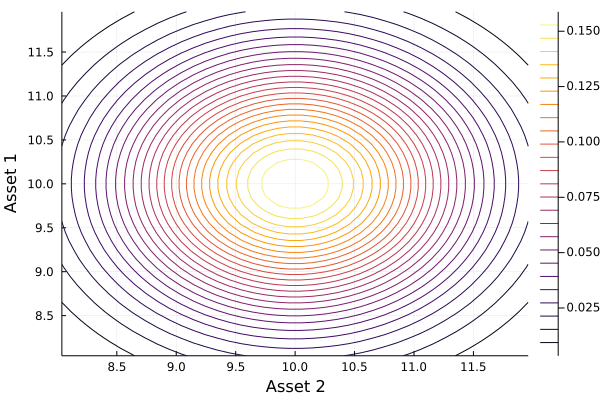
\includegraphics[width=\textwidth]{../plots/params/baseline/prior.png}
        \caption{Baseline}
        \end{subfigure}
    \begin{subfigure}{0.45\textwidth}
        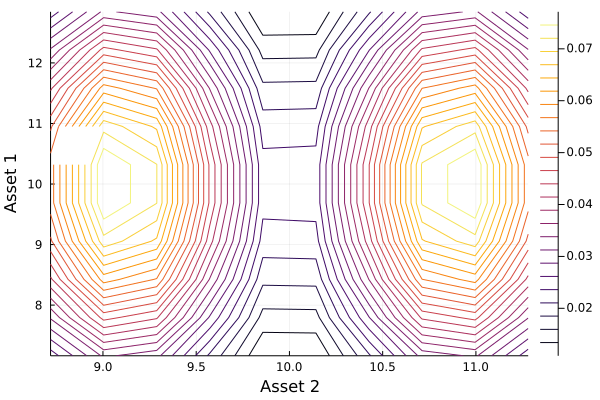
\includegraphics[width=\textwidth]{../plots/params/a2-mean-shift/prior.png}
        \caption{Mean shift}
    \end{subfigure}
    \begin{subfigure}{0.45\textwidth}
        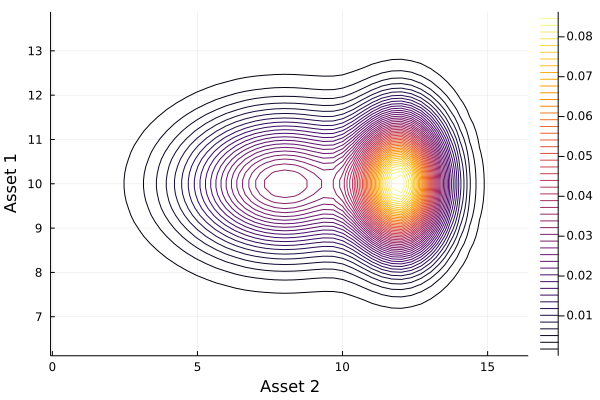
\includegraphics[width=\textwidth]{../plots/params/a2-meanvar-shift/prior.png}
        \caption{Mean and variance shift}
    \end{subfigure}
    \begin{subfigure}{0.45\textwidth}
        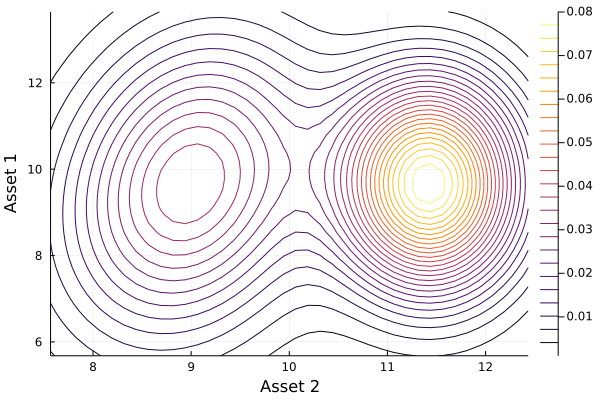
\includegraphics[width=\textwidth]{../plots/params/more-corr-meanvarshift/prior.png}
        \caption{Mean, variance, and correlation shift}
    \end{subfigure}
    \caption{Unconditional joint payoff densities of $f$ in different economies.}
    \label{fig:priors}
\end{figure}

At present, I am most interested in how different attention allocation impacts investor beliefs and asset prices. I fix attention allocation and observe the time-2 portfolio construction problem faced by investors. Later sections will allow agents to optimize their information choices. I generate $J$ agents with $K=1$ attention who equally divide their focus among each asset. Next, I assign each agent a private signal $\eta_j$ based on their attention allocation. I fix the stochastic supply to its average ($x = \bar x$) to more precisely observe equilibrium conditions. Note that the conditions above do not necessarily provide insight about the true qualities of equilibrium in my system, as supply is fixed, and agents are not optimizing their attention allocation.

\subsection{Optimal quantity}

Taking first-order conditions of the portfolio choice problem in \ref{eq:learning-opt} yields the optimal quantity $q^*_j$:

\newcommand{\shat}{\hat s_j}
\newcommand{\hShat}{\hat \Sigma_{H,j}}
\newcommand{\lShat}{\hat \Sigma_{L,j}}
\newcommand{\hMhat}{\hat \mu_{H,j}}
\newcommand{\lMhat}{\hat \mu_{L,j}}
\begin{align}\label{eq:qstar}
    q^*_j = \frac{1}{\rho}\big(\shat \hShat + (1-\shat) \lShat\big)^{-1}\big(\shat \hMhat + (1-\shat) \lMhat - pr \big)
\end{align}

\noindent where $\shat$ represents the posterior probability of being in the high state by investor $j$. It is worth commenting that the form of the optimal quantity is relatively simple and maintains the general form of strict Gaussian case. The only substantive difference between my $q_j$ and that of papers like \textcite{kacperczyk_rational_2016} is that the posterior means and variances are weighted by the posterior state probabilities. The form of $q_j$ demonstrates that it is trivial to add an arbitrary number of Gaussian clusters to the payoff density, should a modeler wish to approximate increasingly complex joint distributions.

\subsection{Prices}

Prices are determined through numerical minimization of the squared difference of the economy from market clearing at a particular draw of payoffs $f$. Denote the total quantity demanded by investors at price $p$ as $\mathbf{q}(p) = q_1(p) + q_2(p) + \dots q_J(p)$.

\begin{mini}
    {A,B,C}{\big(\mathbf{q}(p) - x\big)'\big(\mathbf{q}(p) - x\big)}
    {\label{eq:numerical-opt}}{}
    \addConstraint{p}{= A + B f + C x}
\end{mini}

The optimizer will conjecture price parameters $A$, $B$, and $C$, and then calculate all investor's posterior beliefs about the means, variances, and state probabilities conditional on the particular draw of price parameters. If the price parameters are such that net quantities $\mathbf{q}(p) - x$ is highly positive or negative, the conjectured price function cannot be the market clearing price as there exists some assets which are not held by anyone. I use the LBFGS algorithm with automatic differentiation for the gradient. Typically, the numerical approach yields a squared quantity disjoint around $1e^{-22}$, which is approximately exact for most numerical purposes.

\begin{figure}
    \centering
    \begin{subfigure}{0.45\textwidth}
        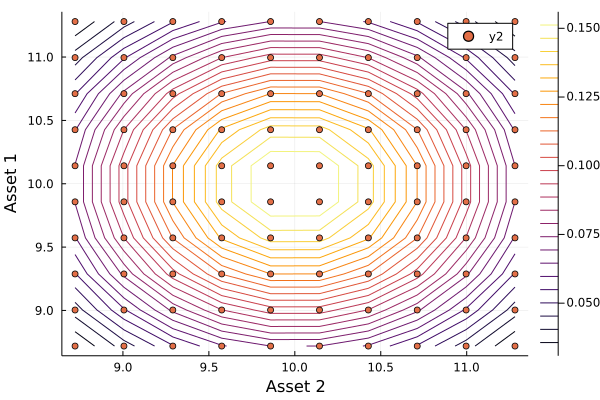
\includegraphics[width=\textwidth]{../plots/params/baseline/prior-grid.png}
        \caption{Baseline}
        \end{subfigure}
    \begin{subfigure}{0.45\textwidth}
        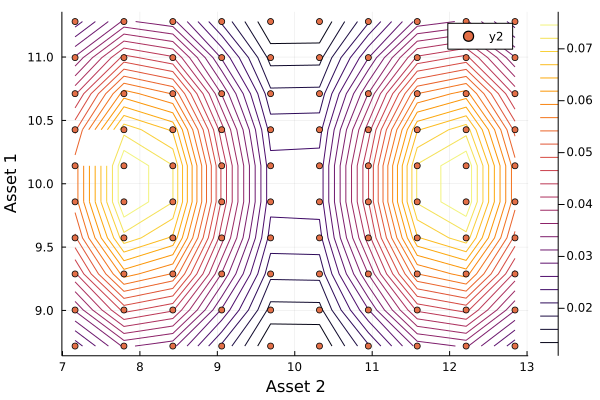
\includegraphics[width=\textwidth]{../plots/params/a2-mean-shift/prior-grid.png}
        \caption{Mean shift}
    \end{subfigure}
    \begin{subfigure}{0.45\textwidth}
        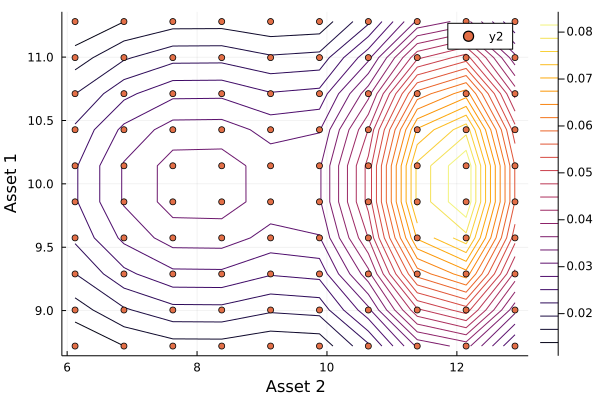
\includegraphics[width=\textwidth]{../plots/params/a2-meanvar-shift/prior-grid.png}
        \caption{Mean and variance shift}
    \end{subfigure}
    \begin{subfigure}{0.45\textwidth}
        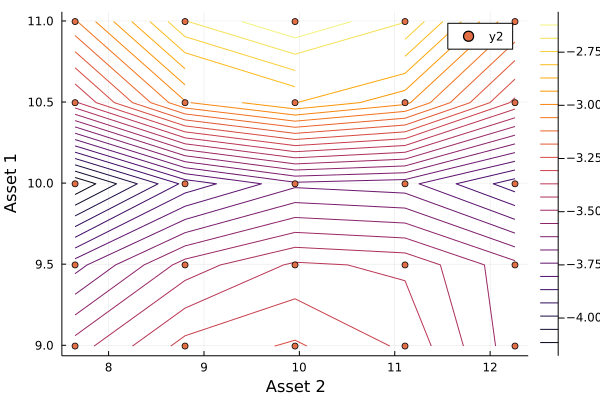
\includegraphics[width=\textwidth]{../plots/params/more-corr-meanvarshift/prior-grid.png}
        \caption{Mean, variance, and correlation shift}
    \end{subfigure}
    \caption{Grid points sampled across the payoff prior density $f$.}
    \label{fig:prior-grid}
\end{figure}


I solve for the market clearing price for each point on a $10 \times 10$ grid of payoffs drawn from the prior density of the economy. Figure \ref{fig:prior-grid} illustrates grid points sampled on each of the four economies. Since I assume that there is a linear price around each payoff grid point but make no aggregate restrictions across pricing functions, the resulting price function tends towards non-linearity. Economies 1 and 2 have strictly linear pricing functions when solving for prices jointly across all grid points, but the introduction of any correlation between assets in different states cannot be numerically solved. This implies that any analytic pricing function I choose must be non-linear\footnote{One possible analytic form for prices might be an $M$-order polynomial in the non-central moments of $f$:

$$
p(f, x) = \sum_{m=0}^M \Phi_m f^m + C x 
$$

This form is attractive, since the non-central moments of each Gaussian component are well-defined. However, investors who observe a price function inclusive of higher moments have significantly more complicated posterior beliefs.
}.

\begin{table}
    \caption{Second-order polynomial approximations to the estimated pricing functions. $a$ represents the intercept term of the polynomial. Standard errors are exceptionally small (as is common in polynomial projections) and are suppressed.}
    \label{tab:poly}
    \begin{tabular}{lcccccc}
        \toprule
        $p_1$ &          $a$ &        $f_1$ &      $f_1^2$ &        $f_2$ &      $f_2^2$ & $f_1\times f_2$\\
     baseline & $        2.66$ & $        0.56$ & $       -0.00$ & $        0.31$ & $       -0.01$ & $       -0.01$\\
a2-mean-shift & $        4.14$ & $        0.50$ & $        0.00$ & $        0.17$ & $       -0.00$ & $       -0.01$\\
a2-meanvar-shift & $        1.31$ & $        0.96$ & $       -0.02$ & $        0.25$ & $       -0.01$ & $       -0.01$\\
more-corr-meanvarshift & $        0.50$ & $        0.84$ & $        0.00$ & $        0.49$ & $       -0.01$ & $       -0.03$\\
\midrule
        $p_2$ &          $a$ &        $f_1$ &      $f_1^2$ &        $f_2$ &      $f_2^2$ & $f_1\times f_2$\\
     baseline & $        2.68$ & $        0.31$ & $       -0.00$ & $        0.56$ & $       -0.00$ & $       -0.01$\\
a2-mean-shift & $        0.42$ & $        0.18$ & $       -0.00$ & $        0.80$ & $       -0.00$ & $        0.00$\\
a2-meanvar-shift & $       -3.86$ & $        0.16$ & $       -0.01$ & $        1.80$ & $       -0.06$ & $        0.01$\\
more-corr-meanvarshift & $       -4.13$ & $        0.58$ & $       -0.02$ & $        1.38$ & $       -0.03$ & $       -0.01$\\
\bottomrule
    \end{tabular}
\end{table}

Table \ref{tab:poly} summarizes the estimated pricing functions using a polynomial basis approximation. Each entry is the coefficient on the quantity in the column. Table \ref{tab:poly} helps capture the fundamental shape of the pricing function of each asset. Some standard findings apply, in that asset prices are increasing in their own payoffs and generally decreasing in their variance. The negative coefficient on the cross term $f_1 \times f_2$ for asset 1 is consistent with the conclusions of consumption models where high consumption state prices are less sensitive to payoffs. In general, however, the riskier asset 2 is more sensitive to payoffs than is asset 1 across all economies.

\subsection{The attention allocation decision}

With prices available, I can turn to the attention allocation decision. Deciding the optimal ex-ante attention allocation requires understanding the distribution of variance-weighted differences in payoffs and prices. In \textcite{kacperczyk_rational_2016}, the authors derive a closed-form linear price as a function of payoffs $f$ and supply shocks $x$, which allowed the authors to define the ex-ante distribution of expected utility as a non-central $\chi^2$ distribution. Unforunately, I do not have a linear price, but I can still characterize investors' optimal attention allocation decision by simulating payoffs, prices, and private signals.

I simulate the distribution of time 1 utility in (\ref{eq:portfolio-opt}), which can be rewritten using optimal quantities of (\ref{eq:qstar}):

\begin{align}\label{eq:exante}
    E[U_{j2}] = r W_0 + \frac{1}{2} E_1\bigg[ E_j[f - pr]'\big(\shat \hShat + (1-\shat) \lShat\big)^{-1}E_j[f - pr] \bigg]
    % \frac{1}{\rho}\big(\shat \hShat + (1-\shat) \lShat\big)^{-1}\big(\shat \hMhat + (1-\shat) \lMhat - pr \big)
\end{align}

Next, I calculate the utility an investor would receive in each state of the world for a different "portfolio" of attention allocation. Note that (\ref{eq:exante}) is an implicit function of the attention matrix $\Sigma_j$. Define the function $\phi(\theta_k) = E[U_{j2}(\theta_k)]$ where $\theta_k \in [0,1]$ indicates the proportion of attention allocated to asset 1, and $1-\theta_k$ indicates the attention allocated to asset 2. The next section attempts to interpret the attention allocation function $\phi(\theta_k)$. $\phi(\theta_k)$ summarizes the ex-ante optimization problem faced by investors.

\section{Analysis}\ref{sec:analysis}

\begin{figure}
    \centering
    \begin{subfigure}{0.45\textwidth}
        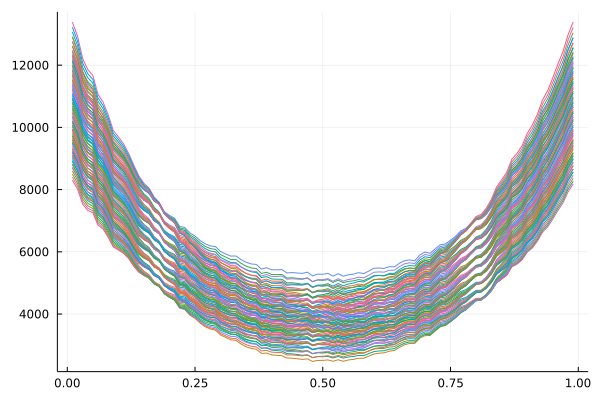
\includegraphics[width=\textwidth]{../plots/params/baseline/optimality_functions.png}
        \caption{Baseline}
    \end{subfigure}
    \begin{subfigure}{0.45\textwidth}
        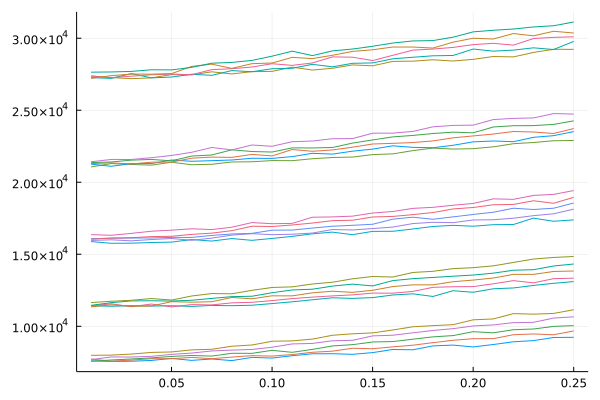
\includegraphics[width=\textwidth]{../plots/params/a2-mean-shift/optimality_functions.png}
        \caption{Mean shift}
    \end{subfigure}
    \begin{subfigure}{0.45\textwidth}
        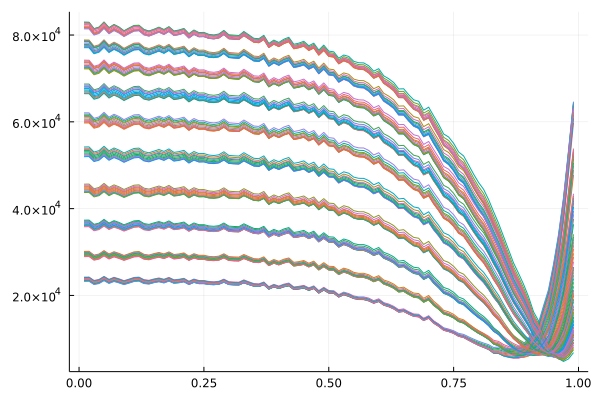
\includegraphics[width=\textwidth]{../plots/params/a2-meanvar-shift/optimality_functions.png}
        \caption{Mean and variance shift}
    \end{subfigure}
    \begin{subfigure}{0.45\textwidth}
        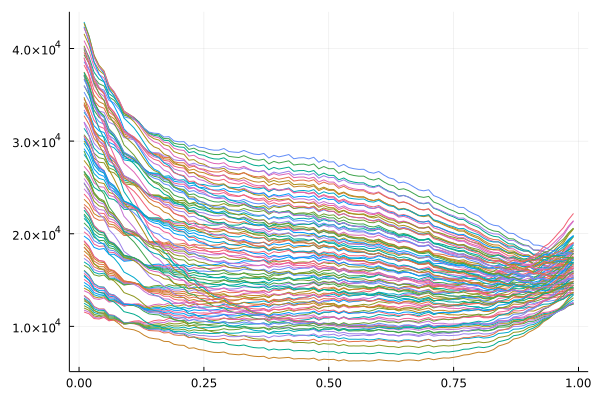
\includegraphics[width=\textwidth]{../plots/params/more-corr-meanvarshift/optimality_functions.png}
        \caption{Mean, variance, and correlation shift}
    \end{subfigure}
    \caption{Plots of the ex-ante utility function $\phi(\theta_k)$ for each grid point $f$.}
    \label{fig:optimality_functions}
\end{figure}

The attention allocation function $\phi(\theta_k)$ is plotted in Figure \ref{fig:optimality_functions}, assuming that all other investors choose $\phi(0.5)$. An investor in a two-asset economy will select $\theta_k$ to maximize $\phi(\theta_k)$. As in \textcite{kacperczyk_rational_2016}, the investor's optimal strategy is usually to allocate all or none of their attention to any particular asset, though the functions that yield this conclusion in my setting are not as simplistic. 

All four panels of Figure \ref{fig:optimality_functions} indicate that the optimal attention allocation decision is on the basis of the \textit{substitutibility} of information -- there is value in knowing what others do not. The substitutibility of information in attention models is not new (see \textcite{van_nieuwerburgh_information_2010}).

What is new is that the complementary action (choosing the same information set as others) is no longer a strictly dominated one. In the baseline case in Panel (a), the optimal attention allocation is to set $\theta_k = 0$ or $\theta_k=1$, with the lowest value of $\phi(\theta_k)$ taking place where all other investors are set ($\theta_k = 0.5$). Panels B,C, and D do not share this quadratic form, and this may indicate that some measure of complementary action should be rational when the economy is more complex. My (speculative) conclusion is driven most starkly by the minor "hump" in the center of the functions of Panel (d). The "hump" in the middle indicates that, as other investors allocate their attention to all asset 1 or asset 2, eventually the middle hump will be the highest point and newly allocating investors will choose to cluster with others. Investors may prefer to have similar information sets to others such that they do not trade with the asymmetrically informed. 

Note that Figure \ref{fig:optimality_functions} indicates that the economy is \textbf{not} in equilibrium. The ex-ante utility function $\phi(\theta_k)$ should be a flat function in equilibrium, as otherwise investor $j$ could deviate and choose another $\theta_k$ to maximize their ex-ante utility. A true equilibrium could be found by adjusting the assumption that all other investors set $\phi(0.5)$ to another quantity, and then calculating any particular investor's incentive to deviate\footnote{The numerical solutions to \textcite{kacperczyk_rational_2016} do just this by allocating attention, noting that some investors would deviate, and then reallocating attention until no investors are willing to deviate.}.

\begin{lemma}
    $p^*(f,x)$ is an equilibrium pricing function if there exists a $\hat \theta_k$ for all other investors such that investor $j$ cannot profitability change their ex-ante attention allocation, i.e. $\derivative{\phi(\theta_k)}{\theta_k} = 0$ everywhere.
\end{lemma}

Importantly, Figure \ref{fig:optimality_functions} suggests the possibility that the existence of a symmetric equilibrium where all investors choose the same attention cannot exist for even moderately complex economies\footnote{\textcite{hellwig_knowing_2009} is consistent with my conjecture, in that games with substitutibility produce heterogeneous beliefs.}. The derivative of $\phi(\theta_k)$ for the complex economies (Panels B-D) are non constant at different points, while the baseline economy of \textcite{kacperczyk_rational_2016} in Panel A has equivalent derivatives at all possible payoffs. The lack of symmetric equilibria is important because it rules out simplistic outcomes and necessitates an equilibrium where some informed investors engaging in attention herding behavior, as others attempt to profit by becoming extremely informed about one asset or the other. 

Such an equilibrium has important ramifications for investors who may tend to fall into one group in the other -- for example, risk-averse funds may herd while more risk-tolerant funds may become asymmetrically informed. In this situation, the risk-tolerant funds would extract an attention-based rent from risk-averse funds. Aggregate disagreement about economic conditions will also be higher as distinct groups select different attention portfolios. More generally, my interpretations of the above indicate a complex economy would produce (a) specialists who understand asset individual payoffs well, and (b) generalists who attempt to consolidate the specialists' information from prices.



It may further be the case that a sufficiently complex economy can no longer support informative prices. Previous works (\textcite{admati_noisy_1985, hellwig1980, kacperczyk_rational_2016} among many others) generally conclude that prices yield information to investors and enhance the welfare value of accurate market prices. The difficulty with this is that, as prior payoffs become more and more complex, the information channel capacity of prices to convey payoff information shrinks. The combination of heterogeneous agent beliefs and uninformative prices mean that prices could exhibit severe excess volatility and disjointed expected returns even with a continuum of rational Bayesian agents. 

\begin{figure}
    \centering
    \begin{subfigure}{0.4\textwidth}
        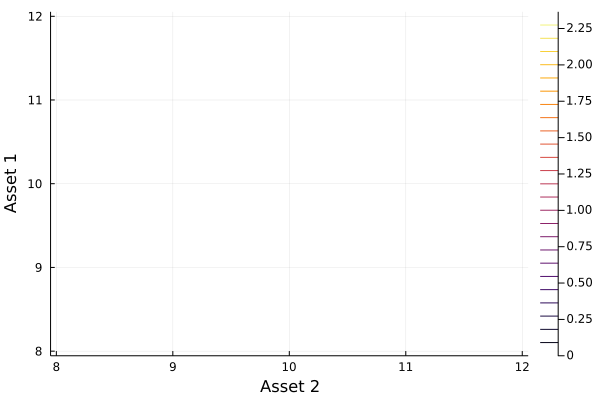
\includegraphics[width=\textwidth]{../plots/params/baseline/entropy_upper.png}
        \caption{Baseline}
    \end{subfigure}
    \begin{subfigure}{0.4\textwidth}
        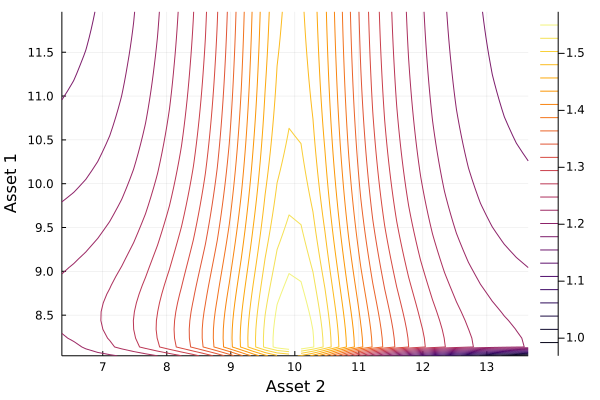
\includegraphics[width=\textwidth]{../plots/params/a2-mean-shift/entropy_upper.png}
        \caption{Mean shift}
    \end{subfigure}
    \begin{subfigure}{0.4\textwidth}
        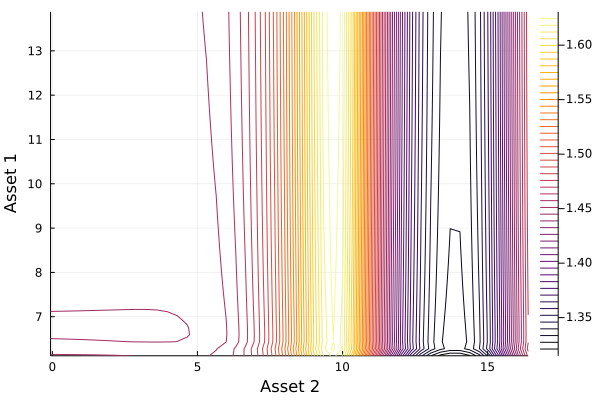
\includegraphics[width=\textwidth]{../plots/params/a2-meanvar-shift/entropy_upper.png}
        \caption{Mean and variance shift}
    \end{subfigure}
    \begin{subfigure}{0.4\textwidth}
        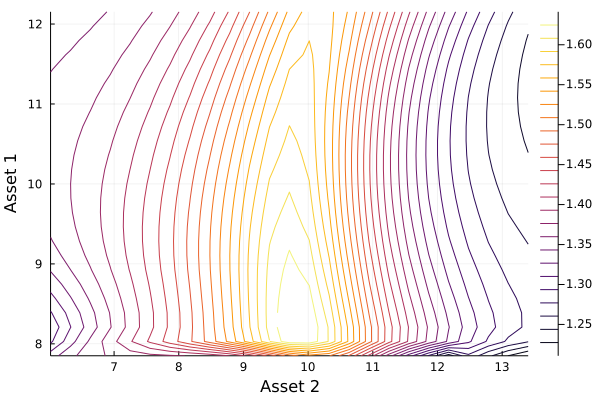
\includegraphics[width=\textwidth]{../plots/params/more-corr-meanvarshift/entropy_upper.png}
        \caption{Mean, variance, and correlation shift}
    \end{subfigure}
    \caption{Distributions of the upper bound on posterior entropy for different observations of $f$. Higher values indicate that investors have increased amounts of irreducible uncertainty. Note that for the multimodal economies, payoffs at the expected value of $[10,10]'$ are also those that have the highest posterior entropy.}
    \label{fig:entropy_upper}
\end{figure}

Prices may be too small a channel to convey exact information (in a NREE sense) in complex economies. In the baseline economy of Section \ref{sec:peq}, the unconditional expected payoff of $E[f] = [10,10]'$ happens to coincide with the distributional mode of $[10,10]'$. The "average" payoff is also the modal payoff, so investors are not particularly uncertain when they observe prices that are indicative of the typical payoff. In a more complicated joint density, prices that indicate the "mean" payoff of $[10,10]'$ can fall in low-density regions between conditional state densities. In this case, the "typical" price is one of the least informative prices possible, since it conveys little information about which state investors are in. 

Figure \ref{fig:entropy_upper} displays the average upper bound on posterior entropy for investors at each grid point in the prior. Note that entropy is highest at the distributional mean for the complex economies, while it is smooth for the baseline economy \footnote{The bound is actually flat everywhere in the baseline case, but Figure \ref{fig:entropy_upper} is technically a bound and may not illustrate this effect. See Figure \ref{fig:entropy_lower} in the appendix for the lower bound on entropy, which illustrates that the baseline economy has constant posterior entropy.}. Put differently, prices that are ex-ante easily expected are also prices that convey the least amount of information. This may not be surprising, but note that forecast errors are \textit{highest} at the mean price in a complex economy, but \textit{lowest} at the mean price in the baseline economy. As the number of economic states increases, it becomes impossible to see how prices can convey any information at all even if prices are functions of the true payoffs.

Regardless, the (temporary) lack of a formal equilibrium and closed-form solution restrict my ability to understand attention allocation across complex economies. Early numerical results are indicative of a non-trivial departure from basic information choice models, in that it is not always optimal to specialize, prices may be highly uninformative, and investor disagreement may play a larger role in observed asset dynamics. In future revisions of this paper, I intend to fully characterize equilibrium conditions, derive more interpretable pricing functions, and form general conclusions about the optimal attention allocation portfolio as a function of the parameters of the prior joint density.

\newpage
\printbibliography

\newpage
\appendix
\pagebreak

\section{Figures}

\begin{figure}
    \centering
    \begin{subfigure}{0.4\textwidth}
        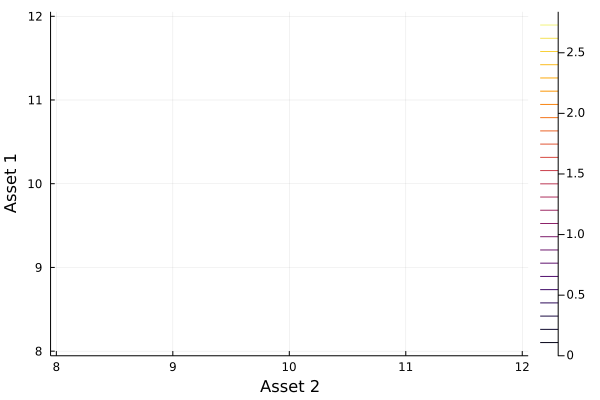
\includegraphics[width=\textwidth]{../plots/params/baseline/entropy_lower.png}
        \end{subfigure}
    \begin{subfigure}{0.4\textwidth}
        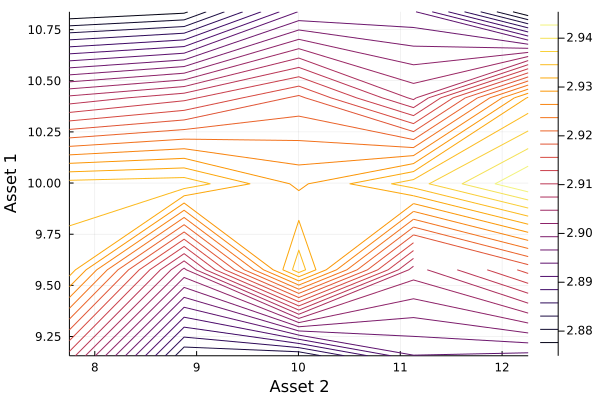
\includegraphics[width=\textwidth]{../plots/params/a2-mean-shift/entropy_lower.png}
    \end{subfigure}
    \begin{subfigure}{0.4\textwidth}
        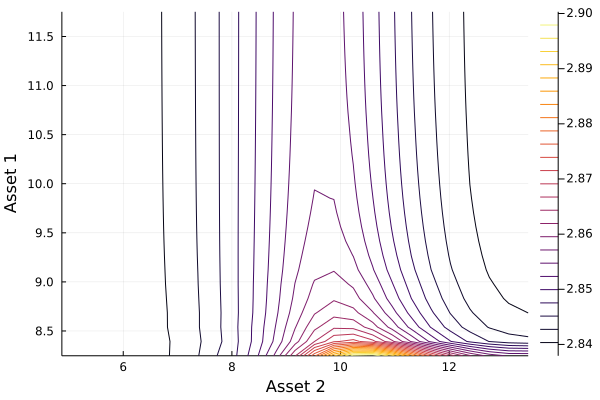
\includegraphics[width=\textwidth]{../plots/params/a2-meanvar-shift/entropy_lower.png}
    \end{subfigure}
    \begin{subfigure}{0.4\textwidth}
        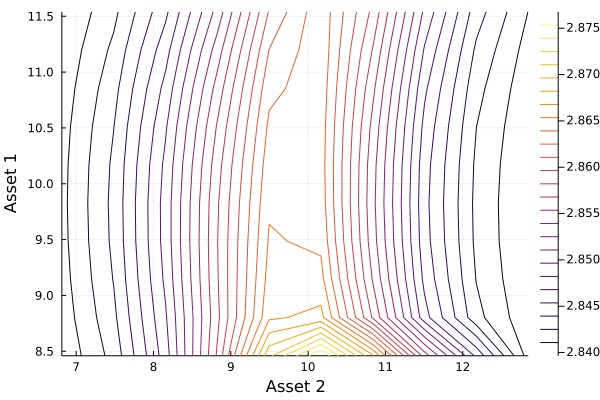
\includegraphics[width=\textwidth]{../plots/params/more-corr-meanvarshift/entropy_lower.png}
    \end{subfigure}
    \caption{Distributions of the lower bound on posterior entropy for different observations of $f$.}
    \label{fig:entropy_lower}
\end{figure}




\begin{figure}
    \centering
    \begin{subfigure}{0.4\textwidth}
        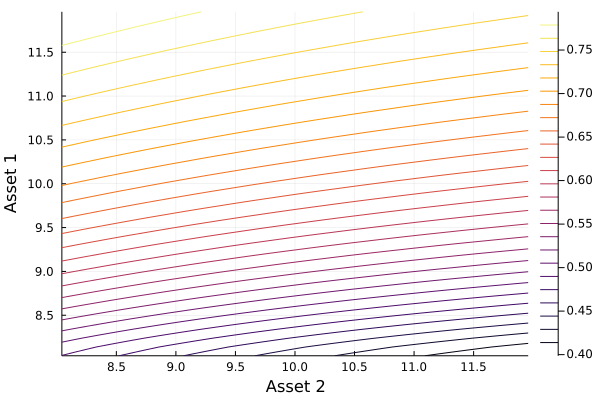
\includegraphics[width=\textwidth]{../plots/params/baseline/b11.png}
        \end{subfigure}
    \begin{subfigure}{0.4\textwidth}
        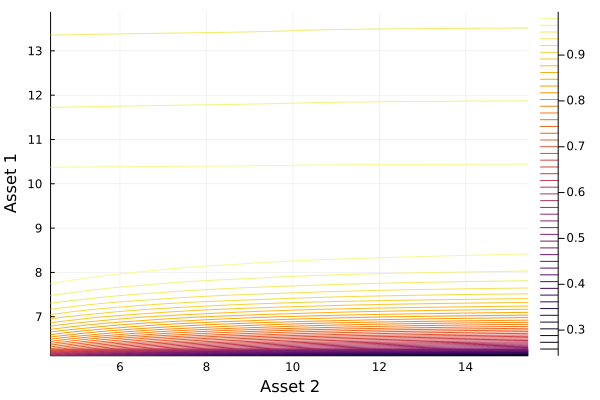
\includegraphics[width=\textwidth]{../plots/params/a2-mean-shift/b11.png}
    \end{subfigure}
    \begin{subfigure}{0.4\textwidth}
        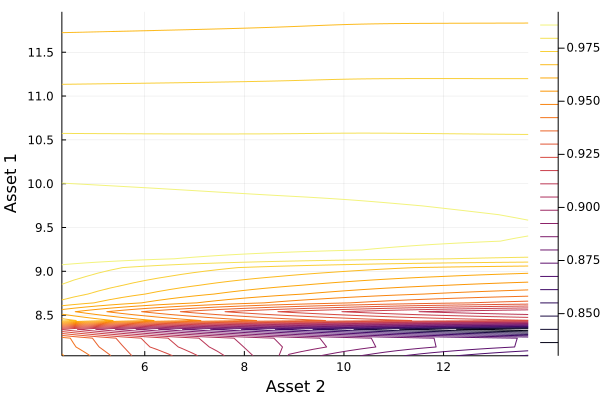
\includegraphics[width=\textwidth]{../plots/params/a2-meanvar-shift/b11.png}
    \end{subfigure}
    \begin{subfigure}{0.4\textwidth}
        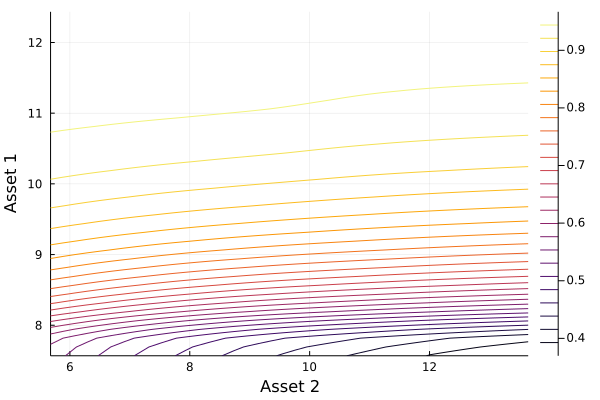
\includegraphics[width=\textwidth]{../plots/params/more-corr-meanvarshift/b11.png}
    \end{subfigure}
    \caption{Distributions of payoff coefficient matrix $B_{1,1}$ for different observations of $f$.}
    \label{fig:b11}
\end{figure}

\begin{figure}
    \centering
    \begin{subfigure}{0.4\textwidth}
        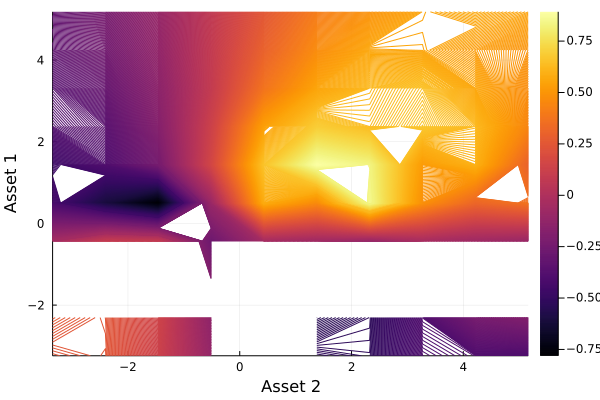
\includegraphics[width=\textwidth]{../plots/params/baseline/b22.png}
        \end{subfigure}
    \begin{subfigure}{0.4\textwidth}
        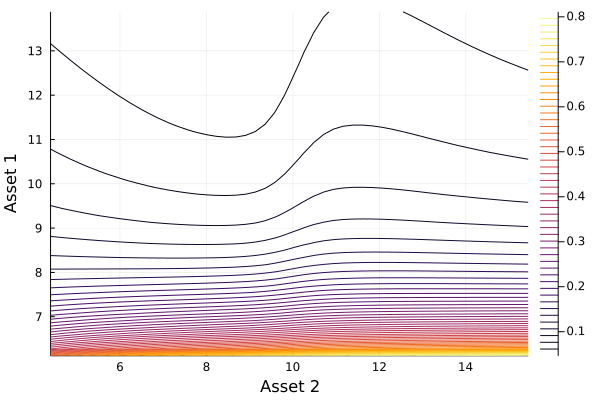
\includegraphics[width=\textwidth]{../plots/params/a2-mean-shift/b22.png}
    \end{subfigure}
    \begin{subfigure}{0.4\textwidth}
        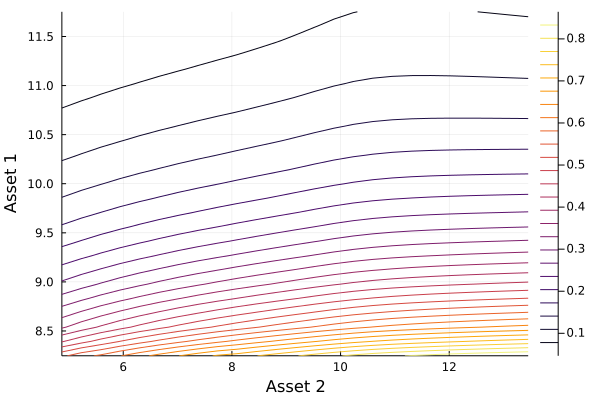
\includegraphics[width=\textwidth]{../plots/params/a2-meanvar-shift/b22.png}
    \end{subfigure}
    \begin{subfigure}{0.4\textwidth}
        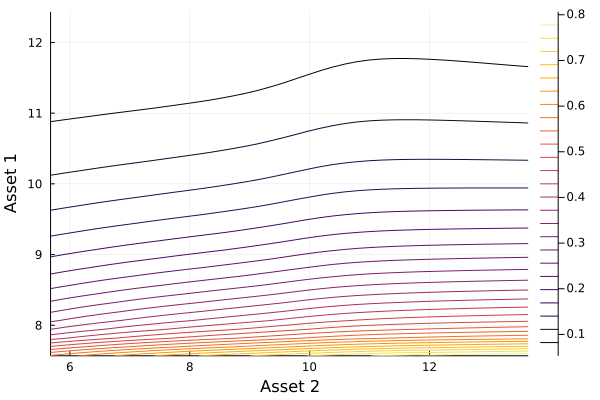
\includegraphics[width=\textwidth]{../plots/params/more-corr-meanvarshift/b22.png}
    \end{subfigure}
    \caption{Distributions of payoff coefficient matrix $B_{2,2}$ for different observations of $f$.}
    \label{fig:b22}
\end{figure}

\begin{figure}
    \centering
    \begin{subfigure}{0.4\textwidth}
        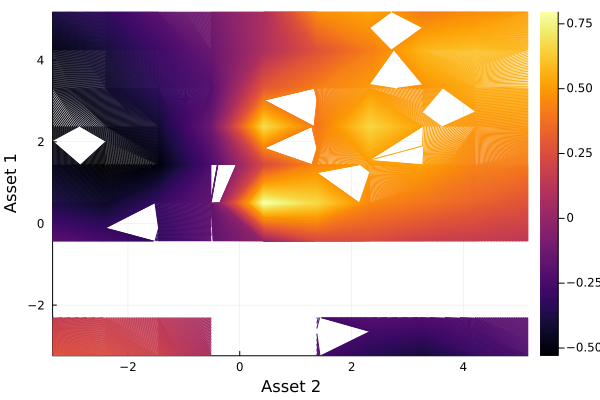
\includegraphics[width=\textwidth]{../plots/params/baseline/b12.png}
        \end{subfigure}
    \begin{subfigure}{0.4\textwidth}
        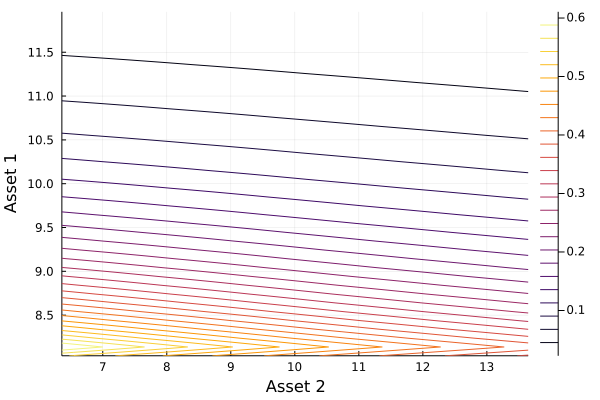
\includegraphics[width=\textwidth]{../plots/params/a2-mean-shift/b12.png}
    \end{subfigure}
    \begin{subfigure}{0.4\textwidth}
        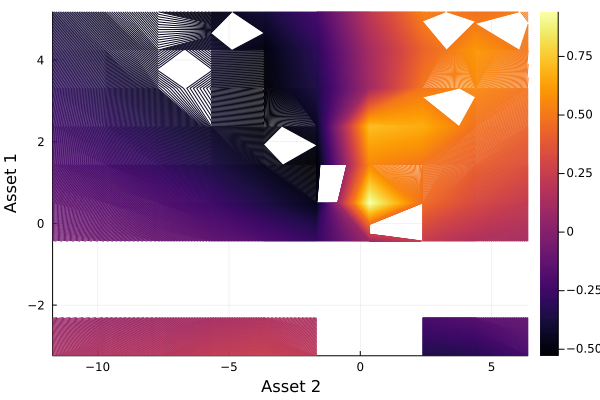
\includegraphics[width=\textwidth]{../plots/params/a2-meanvar-shift/b12.png}
    \end{subfigure}
    \begin{subfigure}{0.4\textwidth}
        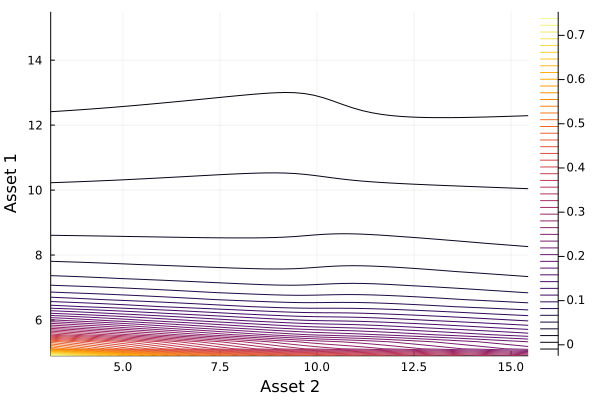
\includegraphics[width=\textwidth]{../plots/params/more-corr-meanvarshift/b12.png}
    \end{subfigure}
    \caption{Distributions of payoff coefficient matrix $B_{1,2}$ for different observations of $f$.}
    \label{fig:b12}
\end{figure}

\begin{figure}
    \centering
    \begin{subfigure}{0.4\textwidth}
        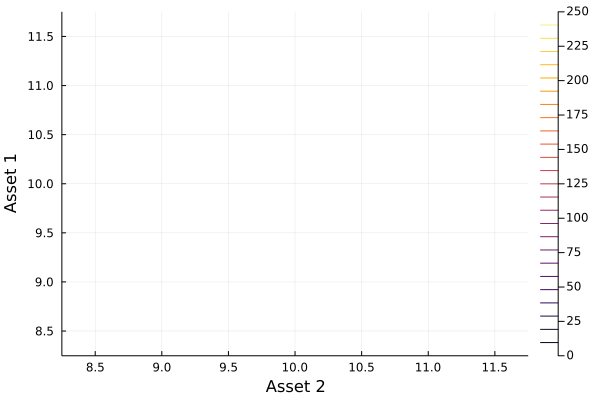
\includegraphics[width=\textwidth]{../plots/params/baseline/disagreement.png}
        \end{subfigure}
    \begin{subfigure}{0.4\textwidth}
        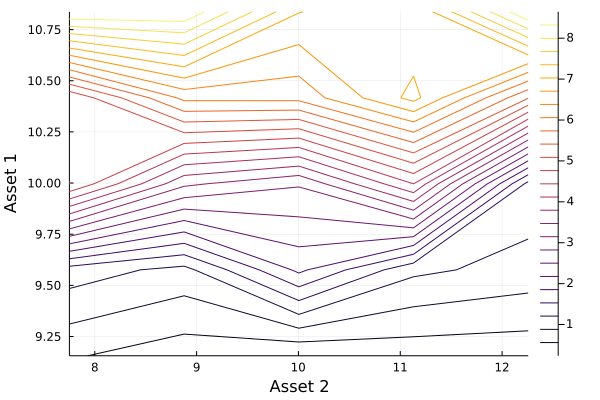
\includegraphics[width=\textwidth]{../plots/params/a2-mean-shift/disagreement.png}
    \end{subfigure}
    \begin{subfigure}{0.4\textwidth}
        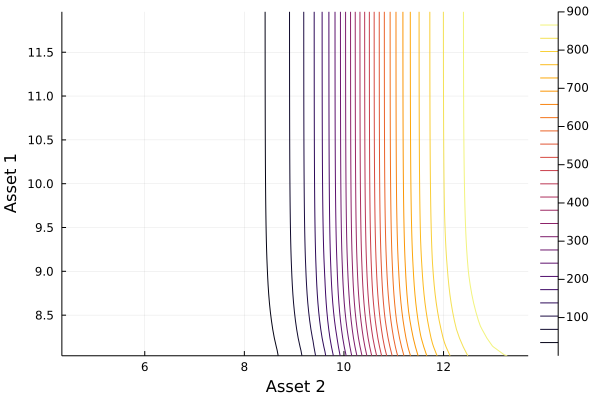
\includegraphics[width=\textwidth]{../plots/params/a2-meanvar-shift/disagreement.png}
    \end{subfigure}
    \begin{subfigure}{0.4\textwidth}
        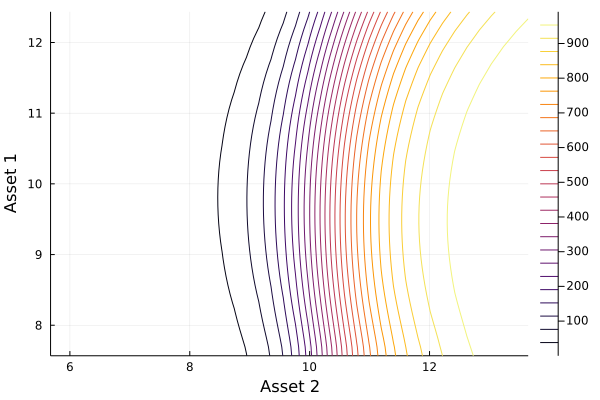
\includegraphics[width=\textwidth]{../plots/params/more-corr-meanvarshift/disagreement.png}
    \end{subfigure}
    \caption{Distributions of disagreement ($\sum \hat s_j^2$) for different observations of $f$.}
    \label{fig:disagreement}
\end{figure}

\begin{figure}
    \centering
    \begin{subfigure}{0.4\textwidth}
        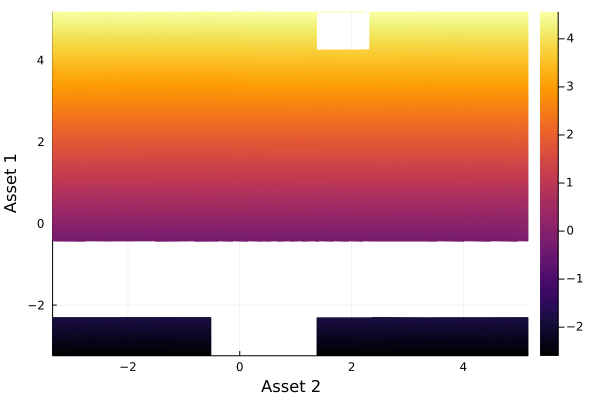
\includegraphics[width=\textwidth]{../plots/params/baseline/p1.png}
        \end{subfigure}
    \begin{subfigure}{0.4\textwidth}
        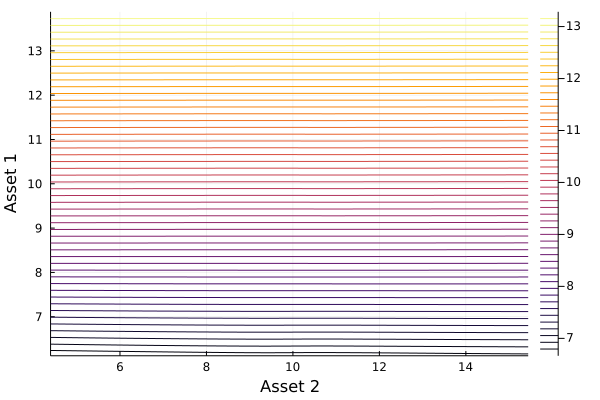
\includegraphics[width=\textwidth]{../plots/params/a2-mean-shift/p1.png}
    \end{subfigure}
    \begin{subfigure}{0.4\textwidth}
        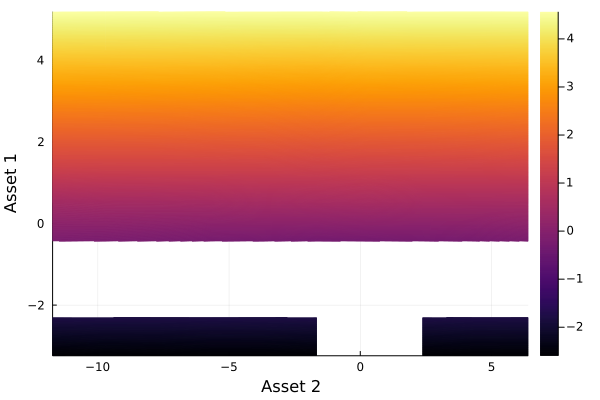
\includegraphics[width=\textwidth]{../plots/params/a2-meanvar-shift/p1.png}
    \end{subfigure}
    \begin{subfigure}{0.4\textwidth}
        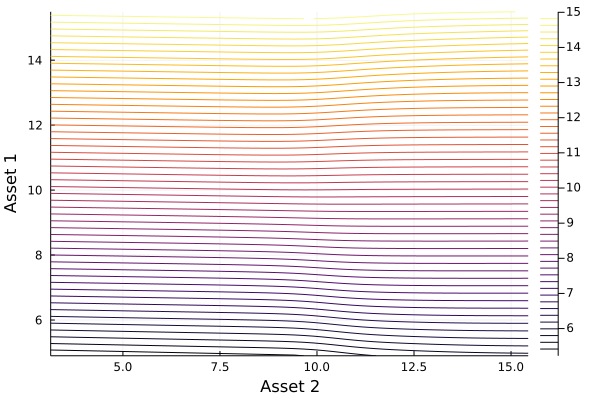
\includegraphics[width=\textwidth]{../plots/params/more-corr-meanvarshift/p1.png}
    \end{subfigure}
    \caption{Distributions of the asset 1 price for different observations of $f$.}
    \label{fig:p1}
\end{figure}

\begin{figure}
    \centering
    \begin{subfigure}{0.4\textwidth}
        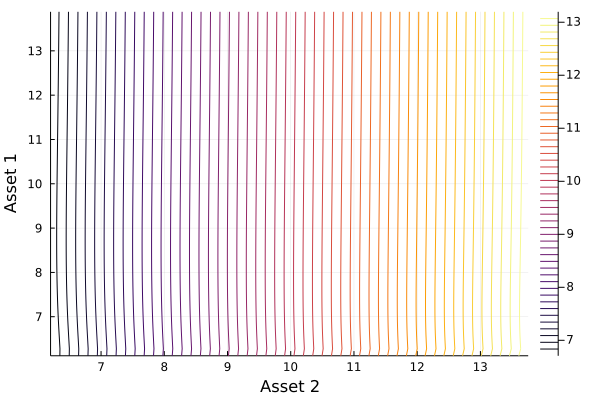
\includegraphics[width=\textwidth]{../plots/params/baseline/p2.png}
        \end{subfigure}
    \begin{subfigure}{0.4\textwidth}
        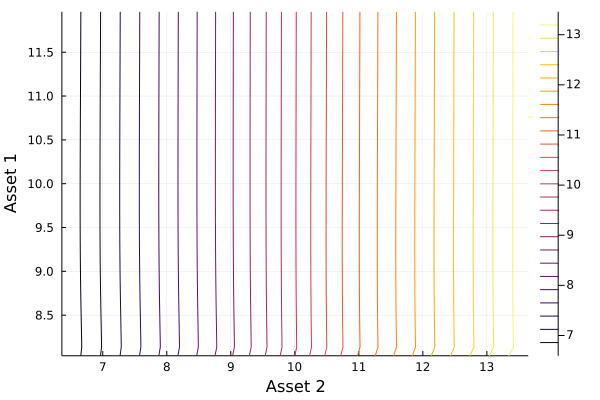
\includegraphics[width=\textwidth]{../plots/params/a2-mean-shift/p2.png}
    \end{subfigure}
    \begin{subfigure}{0.4\textwidth}
        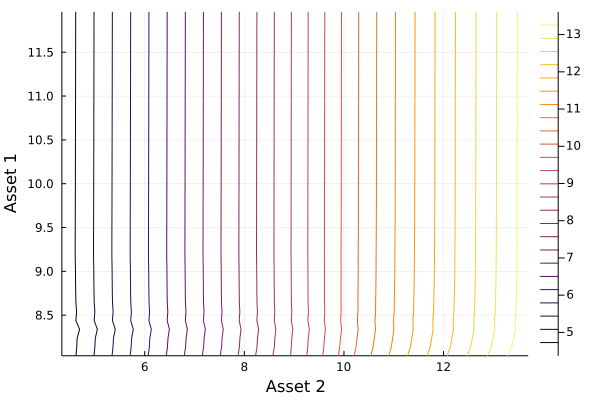
\includegraphics[width=\textwidth]{../plots/params/a2-meanvar-shift/p2.png}
    \end{subfigure}
    \begin{subfigure}{0.4\textwidth}
        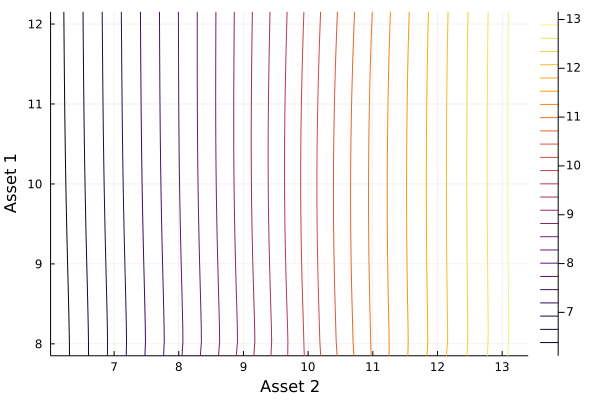
\includegraphics[width=\textwidth]{../plots/params/more-corr-meanvarshift/p2.png}
    \end{subfigure}
    \caption{Distributions of the asset 2 price for different observations of $f$.}
    \label{fig:p2}
\end{figure}



% \begin{figure}
%     \centering
%     \begin{subfigure}{0.4\textwidth}
%         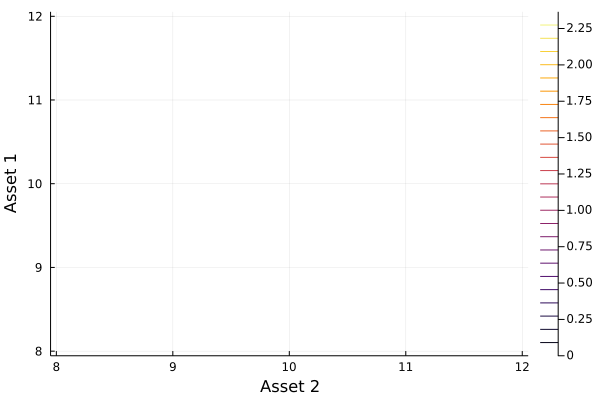
\includegraphics[width=\textwidth]{../plots/params/baseline/entropy_upper.png}
%         \end{subfigure}
%     \begin{subfigure}{0.4\textwidth}
%         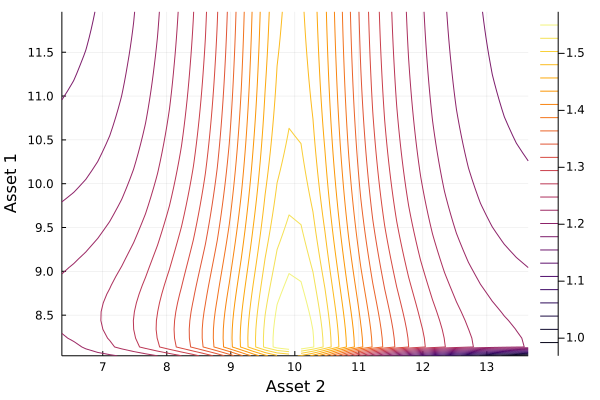
\includegraphics[width=\textwidth]{../plots/params/a2-mean-shift/entropy_upper.png}
%     \end{subfigure}
%     \begin{subfigure}{0.4\textwidth}
%         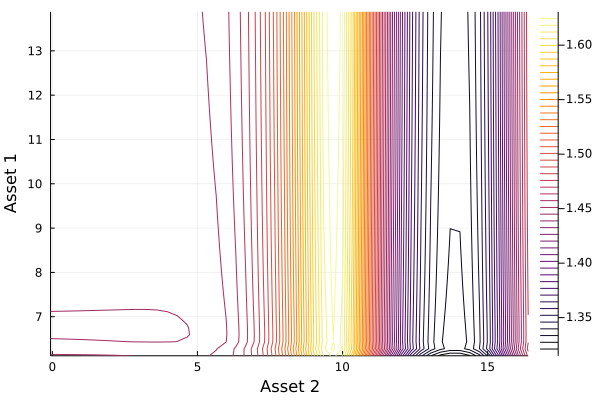
\includegraphics[width=\textwidth]{../plots/params/a2-meanvar-shift/entropy_upper.png}
%     \end{subfigure}
%     \begin{subfigure}{0.4\textwidth}
%         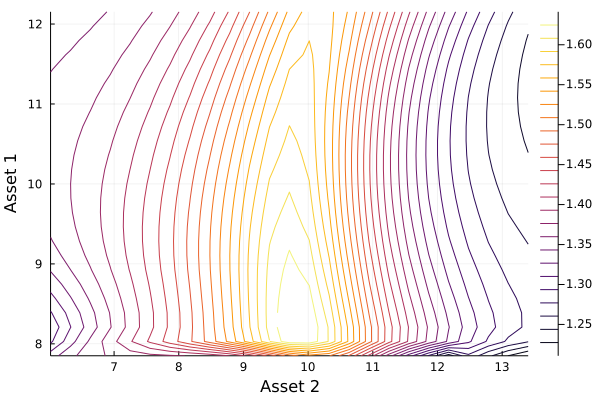
\includegraphics[width=\textwidth]{../plots/params/more-corr-meanvarshift/entropy_upper.png}
%     \end{subfigure}
%     \caption{Distributions of the upper bound on posterior entropy for different observations of $f$.}
%     \label{fig:entropy_upper}
% \end{figure}

\section{Mixture model variance}

The variance-covariance matrix of variable $X$ following a Gaussian mixture distribution with means $\mu = [\mu_1, \mu_2, \dots, \mu_k]'$, covariances $\Sigma= [\Sigma_1, \Sigma_2, \dots, \Sigma_k]$, and mixture proportions $\pi = [\pi_1, \pi_2, \dots, \pi_k]'$ is\footnote{From https://math.stackexchange.com/questions/195911/calculation-of-the-covariance-of-gaussian-mixtures} 

\begin{align}
    \Var[X] &= E[\Var[X \mid k]] + \Var[E[X \mid k]] \\
            &= \sum_k  \pi_k  \bigg(\Sigma_k + (\mu_k - \overline{\mu})(\mu_k - \overline{\mu})' \bigg)
\end{align}

\noindent for $\overline{\mu}=\sum_k \pi_k \mu_k$.

\section{Misc identities}

Stochastic variables:

\begin{itemize}
    \item State variable $s ~ \sim \text{Bernoulli}(\pi)$. $P(s=H) = \pi$, $P(s=L) = 1-\pi$.
    \item Risk factor payoffs $\tilde f \mid s \sim N(\Gamma^{-1} \mu_s, \Sigma_s)$
    \item Risk factor supply $x \sim N(\overline{x}, \sigma_x I)$
    \item Private signals $\eta_j \mid s \sim N(z, \Sigma_{\eta_j})$
    \item Price signal $\eta_p \mid s \sim N(z, \Sigma_p)$
\end{itemize}

Joint density:

$$
P(s, \tilde f, x, \eta_j, \eta_p) = P(\tilde f \mid s) P(\eta_j \mid s) P(\eta_p \mid s) P(s)  P(x)
$$

Posterior density:

$$
P(s, \tilde f \mid x, \eta_j, \eta_p) = 
    \frac{
        P(x, \eta_j, \eta_p \mid s, \tilde f) P(s, \tilde f)
    }{
        P(x, \eta_j, \eta_p)
    }
$$

Unknown values:

\begin{itemize}
    \item $E_j[\tilde f - \tilde p r \mid H]$
    \item $E_j[\tilde f - \tilde p r \mid L]$
    \item $V_j[\tilde f - \tilde p r \mid H]$
    \item $V_j[\tilde f - \tilde p r \mid L]$
    \item $P(H \mid \eta_p, \eta_j)$
    \item $P(L \mid \eta_p, \eta_j)$
    \item $E_j[\tilde f \mid \eta_p, \eta_j]$
    \item $V_j[\tilde f \mid \eta_p, \eta_j]$
    \item $\tilde p$
\end{itemize}

Portfolio choice problem:

\begin{align*}
    U_{2j} &= \max_{\tilde q_j}
        \rho E_j [W_j] - \frac{\rho^2}{2} V_j [W_j] \\
\end{align*}

Optimal quantity:

\begin{align*}
    \tilde q_j &= \frac1\rho \bigg( P(H) \Sigma_H + P(L) \Sigma_L \bigg)^{-1} \bigg(
        P(H) E_j [\tilde f \mid H] + P(L) E_j [\tilde f \mid L] - \tilde p r
    \bigg) \\
    &= \frac1\rho V_j[\tilde f]^{-1} (E_j [\tilde f] - \tilde p r)
\end{align*}

Ex-ante expected utility:

\begin{align*}
    U_{1j} &= E\biggl[
        \rho E_j [W_j] - \frac{\rho^2}{2} V_j [W_j]
    \biggr] \\
    &= 
        \pi E\biggl[
            \rho E_j [W_j \mid H] - \frac{\rho^2}{2} V_j [W_j \mid H]
        \biggr] \\
        &\quad +
        (1-\pi) E\biggl[
            \rho E_j [W_j \mid L] - \frac{\rho^2}{2} V_j [W_j \mid L]
        \biggr] \\
    &= \rho r W_0 \\
        &\quad + 
        \rho \tilde q'_j \biggl(
            \pi E_j [\tilde f - \tilde p r \mid H] +
            (1-\pi) E_j [\tilde f - \tilde p r \mid L]
        \biggr) \\
        &\quad -
        \frac{\rho^2}{2} \tilde q'_j \biggl(
            \pi V_j [\tilde f - \tilde p r \mid H] +
            (1-\pi) V_j [\tilde f - \tilde p r \mid L]
        \biggr) \tilde q_j
\end{align*}


\end{document}
